
%%%%%%%%%%%%%%%%%%%%%%% file typeinst.tex %%%%%%%%%%%%%%%%%%%%%%%%%
%
% This is the LaTeX source for the instructions to authors using
% the LaTeX document class 'llncs.cls' for contributions to
% the Lecture Notes in Computer Sciences series.
% http://www.springer.com/lncs       Springer Heidelberg 2006/05/04
%
% It may be used as a template for your own input - copy it
% to a new file with a new name and use it as the basis
% for your article.
%
% NB: the document class 'llncs' has its own and detailed documentation, see
% ftp://ftp.springer.de/data/pubftp/pub/tex/latex/llncs/latex2e/llncsdoc.pdf
%
%%%%%%%%%%%%%%%%%%%%%%%%%%%%%%%%%%%%%%%%%%%%%%%%%%%%%%%%%%%%%%%%%%%


\documentclass[runningheads,a4paper]{llncs}
\usepackage[margin=0.5in]{geometry}
\usepackage{amssymb}
\setcounter{tocdepth}{3}
\usepackage{graphicx}
\usepackage[polish]{babel}
\usepackage[utf8]{inputenc}
\usepackage{polski}
\usepackage{color}
\usepackage{booktabs}
\usepackage[section]{placeins}

\newcommand{\keywords}[1]{\par\addvspace\baselineskip
\noindent\keywordname\enspace\ignorespaces#1}

\begin{document}
\vspace{-100pt}
\mainmatter  % start of an individual contribution
% first the title is needed
\title{Konstrukcja automatu deterministycznego skończonego sprawdzającego zachodzenie relacji indukowanej przez język dla słów z danego języka (dokumentacja końcowa)\\Teoria algorytmów i obliczeń}

% a short form should be given in case it is too long for the running head
\titlerunning{Dokumetacja końcowa projektu TAIO}

% the name(s) of the author(s) follow(s) next
%
% NB: Chinese authors should write their first names(s) in front of
% their surnames. This ensures that the names appear correctly in
% the running heads and the author index.
%
\author{Anna Zawadzka\and Sylwia Nowak\and Pavel Kuzmich\and Piotr Waszkiewicz}
%
\authorrunning{}
% (feature abused for this document to repeat the title also on left hand pages)

%
% NB: a more complex sample for affiliations and the mapping to the
% corresponding authors can be found in the file "llncs.dem"
% (search for the string "\mainmatter" where a contribution starts).
% "llncs.dem" accompanies the document class "llncs.cls".
%

\toctitle{Lecture Notes in Computer Science}
\tocauthor{Authors' Instructions}
\maketitle

\tableofcontents

\newpage

\section{Wstęp}

\subsection{Cel projektu}

Celem projektu było stworzenie deterministycznego automatu skończonego realizującego funkcję relacji indukowanej przez język na podstawie odpowiedzi udzielanych przez gotowe, nieznane narzędzie pełniące tę samą rolę.

\subsection{Sposób realizacji w etapach}

\begin{itemize}
\item[•] Wprowadzenie narzędzia (automatu), pozwalającego sprawdzić czy $\forall_{x,y \in \Sigma^*} x R_{L} y$
\item[•] Utworzenie treningowego i testowego zbioru słów
\item[•] Znalezienie skończonych automatów deterministycznych spełniających cel projektu z wykorzystaniem algorytmu PSO (Particle Swarm Optimization) i zbioru treningowego słów
\item[•] Wybranie najlepszego utworzonego automatu wykorzystując zbiór testowy słów
\end{itemize}

\newpage

\section{Szczegółowy opis sposobu realizacji zadania}

\subsection{Automat wejściowy}

Na podstawie automatu wejściowego zostało stworzone narzędzie sprawdzające, czy dwa słowa są ze sobą w relacji. Informacje o automacie wejściowym przechowywane są w pliku tekstowym podawanym na wejście programu. Format reprezentacji automatu jest następujący:

\begin{itemize}
\item[•] Stany numerowane liczbami $1, 2, …, n$, gdzie $n$ to liczba stanów, $1$ – stan początkowy
\item[•] $r$ – liczba symboli w alfabecie
\item[•] Tabela funkcji przejścia
\end{itemize}

Po wprowadzeniu pliku z opisem automatu można zobaczyć jego graficzną reprezentację w postaci grafu.

\subsection{Zbiór treningowy i zbiór testowy}

Utworzenie treningowego i testowego zbioru słów nastąpuje poprzez wygenerowanie odpowiednich zbiorów. Są one dostępne (nie zmienią się) dopóki zbiór symboli alfabetu pozostanie ten sam. \\

Zbiór treningowy zawiera wszystkie słowa nad alfabetem o długości mniejszej bądź równej długości podanej przez użytkownika (nie większej niż 5). \\

Zbiór testowy składa się ze słów będących wariacjami bez powtórzeń dla słów o  długości nie mniejszej niż 7 i nie większej niż maksymalna ilość stanów poszukiwanego automatu. W przypadku mniejszej ilości symboli alfabetu niż wymagałyby tego wariacje następuje konstrukcja nowego, tymczasowego zbioru poprzez powielenie wszystkich symboli alfabetu i dodanie ich do istniejących już symboli. Nowe symbole są dodatkowo indeksowane numerem oznaczającym w której iteracji zostały dodane. Zapewnia to ich rozróżnialność podczas konstrukcji zbiorów.\\

Przykład zbioru: {0, 1}. 
Zbiór po przygotowaniu do utworzenia wariacji bez powtórzeń dla słów długości 6: {0, 1, $0_{1}$, $1_{1}$, $0_{2}$, $1_{2}$}. \\

Dodatkowo do zbioru treningowego zostały dodane losowe słowa (zawierające losowe litery alfabetu) o losowej długości z przedziału $[x1,x2]$ , gdzie $x1$ jest maksymalną długością słowa treningowego generowanego poprzednią metodą (przy użyciu wariacji z powtórzeniami) a $x2$ jest nowym parametrem oznaczającym maksymalną długość losowego słowa. W przypadku gdy $x2 < x1$ nie generowane są żadne dodatkowe słowa. Użytkownik może również określić maksymalną ilość słów losowych. Dodatkowo dla każdego nowego słowa $s1$ dopisanego do zbioru treningowego tworzone jest słowo $s2$ tej samej długości lecz również o losowej zawartości, które jest dopisywane do zbioru słów testowych. \\

Zbiór treningowy i testowy są zbiorami rozłącznymi.\\

\subsection{Opis przestrzeni poszukiwania dla algorytmu PSO}

Przestrzeń poszukiwania w algorytmie PSO będą stanowić wszystkie deterministyczne automaty skończone o określonej liczbie stanów, z alfabetem wejściowym równoważnym z alfabetem języka $L$. Zapis cyfrowy każdego automatu można przedstawić jako zbiór macierzy binarnych o wymiarach $|Q|^2$ (gdzie $|Q|$ to ilość stanów automatu). Zbiór ten jest równoliczny ze zbiorem symboli alfabetu automatu (każdemu symbolowi odpowiadać będzie inna macierz). Jeżeli jako dodatkowe założenie przyjmiemy, że w każdym wierszu każdej macierzy znajdować może się tylko jedna jedynka, to wtedy taką macierz traktować możemy jako część tabelki funkcji przejścia automatu, która dla wiersza o numerze i oraz jedynce w kolumnie $j$ odpowiada przejściu ze stanu $q_{i}$ do stanu $q_{j}$ po wczytaniu symbolu przypisanego do tej macierzy. Ponieważ następująca reprezentacja jest nieoptymalna pod względem zużycia pamięci zapis został uproszczony do tablicy jednowymiarowej, która dla każdego indeksu odpowiadającego numerowi stanu w którym automat znajduje się przed wczytaniem symbolu, przyporządkowuje numer stanu w którym automat znajdzie się po wczytaniu elementu z taśmy.\\

Dla przykładu, po zastosowaniu takiej optymalizacji dla tabeli funkcji przejścia 
\begin{table}[]
\centering
\begin{tabular}{c|c|c|c|}
symbol                   & $q_{1}$ & $q_{2}$ & $q_{3}$ \\ \hline
\multicolumn{1}{c|}{$q_{1}$} & 0  & 1  & 0  \\ \hline
\multicolumn{1}{c|}{$q_{2}$} & 1  & 0  & 0  \\ \hline
\multicolumn{1}{c|}{$q_{3}$} & 0  & 0  & 1  \\ \hline
\end{tabular}
\vspace{0.5cm}
\caption{Przykładowa tabela funkcji prześcia}
\end{table}

otrzymamy jako wynik wektor [1 0 2].\\

Przyjmijmy $d = |\Sigma|$ liczba symboli alfabetu, $f = |Q|$ liczba stanów automatu. Tak więc przestrzeń wszystkich automatów stanowią wszystkie możliwe ciągi liczb o długości $d*f$ i wartościach z przedziału $[0, f)$. Cząstki poruszające się w przestrzeni przyjmują pozycje będące reprezentacją tych automatów. Dla każdej cząsteczki jej prędkość definiowana jest jako $V_{p} = (V_{1}, V_{2}, …, V_{d})$, gdzie $V_{i (1 \leq i \leq d)}$ oznacza prędkość cząstki na płaszczyźnie odpowiadającej symbolowi o numerze $i$, definowanej jako $V_{pi} = (V_{1}, V_{2}, …, V_{f})$. $V_{j (1 \leq j \leq f)}$ reprezentuje tutaj prędkość cząstki dla wiersza numer $j$ w macierzy zdefiniowanej wcześnie jako reprezentacja tabeli funkcji przejścia dla danego symbolu. Tak zdefiniowaną prędkość można (podobnie jak położenie) przedstawić w postaci tablicy jednowymiarowej o długości $d*f$ (gdzie $d$ i $f$ - zdefiniowane wcześniej). Zmiana położenia cząstki następuje więc poprzez dodanie wektora prędkości do wektora położenia tym samym otrzymując nowe położenie.

\subsection{Odległość w przeszukiwanej przestrzeni}

Dla tak zdefiniowanej przestrzeni i ciągów liczb długości d*f, które reprezentują automaty została wprowadzona metryka nazywana metryką Hamminga. Dla dwóch ciągów $a$ i $b$ z tej przestrzemi odległość Hamminga jest równa liczbie jedynek w słowie $a XOR b$, np. odległość pomiędzy ciągami 10\textbf{0}11\textbf{1}01 i 10\textbf{1}11\textbf{0}01 wynosi 2.

\subsection{Przeszukiwanie przestrzeni w algorytmie PSO}

Przeszukiwanie przestrzeni automatów realizowane jest poprzez wygenerowanie pewnej ilości cząstek (nazywanych rojem) poruszających się według określonych zasad i dążących do osiągnięcia postawionego celu. Za cel najczęściej przyjmuje się minimalizację wartości pewnej funkcji nazywanej funkcją celu. W tym projekcie jest to funkcja $f:A \rightarrow N$ ($A$ - zbiór automatów, $N$ - liczby naturalne), która dla danego automatu zwraca liczbę błędnie zaklasyfikowanych słów.\\

W trakcie kolejnych kroków zdyskretyzowanego czasu cząstki przemieszczają się do nowych pozycji, symulując adaptację roju do środowiska poszukując optimum. Każda cząstka pamięta swoje dotychczasowe najlepsze położenie (miejsce w przestrzeni gdzie znaleziony automat miał najniższą wartość funkcji celu). “Liderem” roju zostaje ta o najlepszym położeniu z całego roju. Położenia cząstek w obszarze przeszukiwania stanowią potencjalne rozwiązania. \\

Algorytm PSO funkcjonuje według następującego schematu:

\begin{enumerate}
\item Nadanie cząstkom roju losowe położenia
\item Dokonanie oceny położenia cząstek za pomocą funkcji dopasowania (fitness)
\item Zmiana zapisu w pamięci cząstek dotycząca najlepszych własnych położeń
\item Wyłonienie lidera roju
\item Aktualizacja wektora prędkości każdej cząstki

\begin{displaymath}
v[\;] = v[\;] + c1 * rand(\;) * (pbest[\;] - present[\;]) + c2 * rand(\;) * (gbest[\;] - present[\;]) \hspace{15mm} (1)
\end{displaymath}

\item Aktualizacja położenia każdej cząstki - jeżeli położenie nie uległo zmianie przez przynajmniej trzy iteracje losowane zostaje nowe położenie

\begin{displaymath}
present[\;] = present[\;] + v[\;] \hspace{15mm} (2)
\end{displaymath}

gdzie

\begin{itemize}
\item[$present$] -- wektor położenia $i$-tej cząstki,
\item[$v$] -- odpowiedni wektor prędkości danej cząstki,
\item[$pbest$] -- najlepsze dotąd znalezione położenie $i$-tej cząstki,
\item[$gbest$] - najlepsze dotąd znalezione położenie lidera roju,
\item[$c1, c2$] - współczynniki wagowe, określane na poziomie $i$-tej cząstki.
\end{itemize}
\end{enumerate}

Współczynniki $c1, c2$ są ustalonymi mnożnikami wagowymi. Współczynniki  są liczbami losowymi o rozkładzie równomiernym w przedziale [0, 1]. \\

Jeżeli w trakcie działania algorytmu PSO któraś z cząstek nie będzie zyskiwać lepszego położenia przez więcej niż trzy iteracje zostaje jej przydzielone nowe, zupełnie losowe położenie. Dzięki temu zyskuje się lepszą zbieżność do najlepszego automatu, oraz unika ryzyka uwięzienia w lokalnym minimum. Cząstki które w danym ruchu miałyby wyjść poza obszar poszukiwań zamiast być stopowane zostają umieszczone na początku tego obszaru z przeciwległej strony. \\

Punkty 2-6 należy wykonywać w pętli dopóki oba warunki będą spełnione:

\begin{itemize}
\item[•] któraś z cząstek nie osiągnie założonej wartości minimalnej błędu
\item[•] nie zostanie osiągnięta z góry wyznaczona ilość iteracji ruchu.
\end{itemize}

Jeden przebieg pętli odpowiada krokowi czasowemu dla poruszającego się roju. Wartość kroku czasowego przyjmuje się jako jednostkową.
Cząstki poruszają się ruchem odcinkowo prostoliniowym. Postać równań (1) i (2) wynika z drugiej zasady dynamiki Newtona, gdzie wypadkowa siła wywołująca przyspieszenie każdej cząstki powstaje wskutek działania sił od “naciągniętych sprężyn” pomiędzy położeniami aktualnym a najlepszymi położeniami: własnym oraz lidera roju. Kolejny wektor prędkości czasu jest wynikiem jej przyspieszenia w kierunku nowego, potencjalnie lepszego położenia, bazując na stale zmieniających się najlepszych wcześniej znanych położeniach.\\

Dla każdej wartości $i$ = 1, 2, 3, …  algorytm PSO uruchamiany jest w przestrzeni z automatami o $i$ stanach. Warto zwrócić uwagę, że istnieje możliwość znalezienia kilku automatów spełniających warunki zakończenia algorytmu PSO. Aby zminimalizować ryzyko wybrania niewłaściwego automatu, po zakończeniu obliczeń dla każdej wartości parametru $i$ najlepszy automat dla danej ilości stanów jest testowany na zbiorze testowym. Ostateczna decyzja wyboru najlepszego rozwiązania zostaje podjęta na podstawie uzyskanej wartości funkcji celu na tym zbiorze.

\newpage

\FloatBarrier
\section{Wyniki przeprowadzonych testów}

Podczas sprawdzania skuteczności zaproponowanego rozwiązania wykonano szereg następujących testów. \\

Dla wszystkich symulacji przyjęto alfabet pięcioznakowy. Wykonano po 50 iteracji przeszukiwania przestrzeni dla każdej klasy automatów o 4, 6, 10, 15 stanach z losową funkcją przejścia. Dla algorytmu PSO rozważane były przestrzenie automatów z ilością stanów z zakresu 3 - 15. Liczebność roju wynosiła 100 cząsteczek. Zbiór treningowy oraz testowy konstruowane były zgodnie z zasadami przedstawionymi we wcześniejszych sekcjach tego dokumentu. \\

Poniżej zostały przedstawione wyniki eksperymentów. \\

\begin{figure}[!htb]
\minipage{0.7\textwidth}
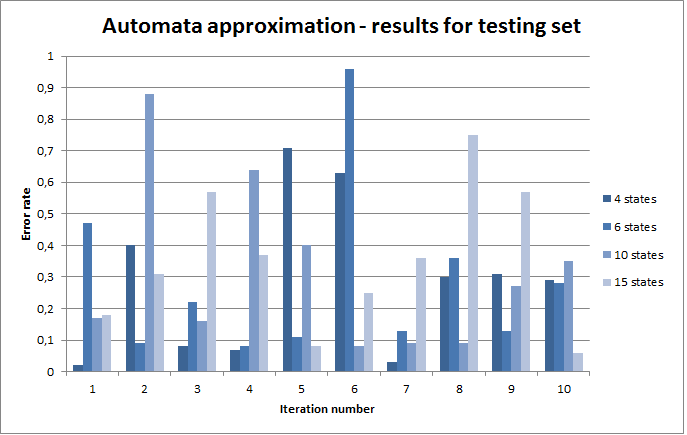
\includegraphics[scale=1]{1.png}
\endminipage\hfill
\minipage{0.8\textwidth}
\renewcommand{\arraystretch}{1.5}% Wider
\begin{tabular}{@{}ccccc@{}}
\toprule
        & 4 states & 6 states & 10 states & 15 states \\ \midrule
1       & 0.02     & 0.47     & 0.17      & 0.18      \\
2       & 0,4      & 0,09     & 0,88      & 0,31      \\
3       & 0,08     & 0,22     & 0,16      & 0,57      \\
4       & 0,07     & 0,08     & 0,64      & 0,37      \\
5       & 0.71     & 0.11     & 0.4       & 0.08      \\
6       & 0,63     & 0,96     & 0,08      & 0,25        \\
7       & 0,03     & 0,13     & 0,09      & 0,36        \\
8       & 0,3      & 0,36     & 0,09      & 0,75         \\
9       & 0,31     & 0,13     & 0,27      & 0,57     \\
10      & 0.29     & 0.28     & 0.35      & 0.06      \\ \bottomrule
Average & 0.28    & 0.28    & 0.31     & 0.35      \\ \bottomrule
\end{tabular}
\vspace{4mm}
\endminipage\hfill
\caption{Aproksymacja automatów klasy 4, 6, 10 oraz 15 na zbiorze testowym}
\end{figure}

\begin{figure}[!htb]
\minipage{0.7\textwidth}
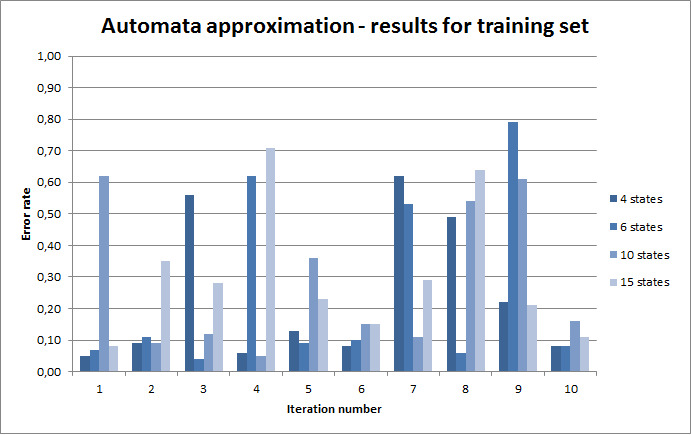
\includegraphics[scale=1]{6.png}
\endminipage\hfill
\minipage{0.8\textwidth}
\renewcommand{\arraystretch}{1.5}% Wider
\begin{tabular}{@{}ccccc@{}}
\toprule
        & 4 states & 6 states & 10 states & 15 states \\ \midrule
1       & 0,05     & 0,07     & 0,62      & 0,08      \\
2       & 0,09     & 0,11     & 0,09      & 0,35      \\
3       & 0,56     & 0,04     & 0,12      & 0,28      \\
4       & 0,06     & 0,62     & 0,05      & 0,71      \\
5       & 0,13     & 0,09     & 0,36      & 0,23      \\
6       & 0,08     & 0,10     & 0,15      & 0,15        \\
7       & 0,62     & 0,53     & 0,11      & 0,29        \\
8       & 0,49     & 0,06     & 0,54      & 0,64         \\
9       & 0,22     & 0,79     & 0,61      & 0,21     \\
10      & 0,08     & 0,08     & 0,16      & 0,11      \\ \bottomrule
Average & 0,24     & 0,25     & 0,28      & 0,31      \\ \bottomrule
\end{tabular}
\vspace{4mm}
\endminipage\hfill
\caption{Aproksymacja automatów klasy 4, 6, 10 oraz 15 na zbiorze treningowym}
\end{figure}

\newpage

\FloatBarrier
\subsection{Skuteczność aproksymacji automatu o 4 stanach}

Aproksymacja automatu o 4 stanach zakończyła się znalezieniem automatu o średnim współczynniku błędu na poziomie 0,24 dla zioru treningowego i 0,28 dla zbioru testowego. Oznacza to, że średnio dla 24 wyrazów (lub odpowiednio 28 wyrazów) na 100 relacja przynależności do tej samej klasy abstrakcji zwróciła błędny wynik. Warto zwrócić uwagę na to, że podczas testów zdarzały się zarówno automaty o bardzo niskim wpółczynniku błędu jak i takie, których wpółczynnik ten był naprawdę wysoki. Zauważono również zależność pomiędzy liczbą iteracji a liczbą błędnie zaklasyfikowanych wyrazów. Wraz ze wzrostem liczby iteracji dla algorytmu PSO wynikowe automaty osiągały o wiele niższe współczynniki dla zbioru treningowego oraz zauważalnie niższe dla zbioru testowego. \\

\FloatBarrier
\subsection{Skuteczność aproksymacji automatu o 6 stanach}

Podobnie jak w przypadku poprzednim współczynnik błędu dla znalezionych automatów zazwyczaj nie przekraczał wartości 0,3. Błędy na poziomie większym niż 0,7 można uznać za błąd gruby. \\

\FloatBarrier
\subsection{Skuteczność aproksymacji automatu o 10 stanach}

W przypadku automatów o 10 stanach wyniki aproksymacji nie odbiegały wiele od wyników z poprzednich prób. Program zwracał dobrze rokujące wyniki, a znalezione automaty zazwyczaj miały podobną ilość stanów co poszukiwany automat. Zauważono zależność, że automaty o liczbie stanów większej bądź równej liczbie stanów poszukiwanego narzędzia charakteryzowały się uzyskiwaniem lepszych (mniejszych) współczynników błędu niż automaty o mniejszej liczbie stanów. \\

\FloatBarrier
\subsection{Skuteczność aproksymacji automatu o 15 stanach}

W przypadku aproksymacji automatów o 15 stanach za pomocą automatów o liczbie stanów z zakresu [3, 15] liczba błędów zaczęła rosnąć. Współczynniki błędu większe niż 0,3 pojawiały się o wiele częściej i można przypuszczać, że pojedynczy wynik 0,8 był dziełem przypadku (wylosowanego automatu wraz z funkcją przejścia). Jedną z prawdopodobnych przyczyn takiego stanu rzeczy była możliwość napotkania automatów o nieosiągalnych stanach podczas przeszukiwania przestrzeni metodą PSO. Automaty takie będące uproszczoną wersją poszukiwanego narzędzia sprawdzającego przynależność do klas abstrakcji nie radzą sobie najlepiej w przypadku wystąpienia dłuższych słow. Ponieważ przestrzeń poszukiwań kończyła się w przestrzeni automatów z 15 stanami, istaniała duża szansa na wylosowanie automatów o niepustym zbiorze stanów nieosiągalnych, a co za tym idzie - na utratę pewnej części informacji o poszukiwanym automacie. Stąd też pogorszenie wyników aproksymacji. \\

\FloatBarrier
\subsection{Dodatkowe próby}
Dalej przeprowadzone zostały próby aproksymacji automatów o 20, 30, 50, 80 stanach przez inne, o mniejszej liczbie stanów - 4, 6, 8, 10, 12. Celem tych eksperymentów było sprawdzenie czy istnieje szansa na upraszczanie skomplikowanych automatów bez utraty (lub małych stratach) informacji o klasach abstrakcji. \\

\FloatBarrier
\subsection{Skuteczność aproksymacji automatu o 20 stanach}

Aproksymacja automatu o 20 stanach automatami o dopowiednio 4, 6, 8, 10 i 12 stanach zakończyła się znalezieniem automatów o średnim współczynniku błędu na poziomie 0,95 dla zbioru treningowego i testowego. Oznacza to, że automaty znalezione nie aproksymują w sposób zadowalający. Warto zauważyć, że dla zbioru treningowego średni współczynnik dla automatów aproksymujących jest prawie stały bez względu na ilość stanów - 0,95. W przeciwieństwie do zbioru treningowego, zbiór testowy posiada średnią aproksymację z przedziału [0,9 1] co oznacza, że prawie dla każdego słowa automat aproksymujący kończył w innym stanie niż automat wejściowy.  \\

\begin{figure}[!htb]
\minipage{0.5\textwidth}
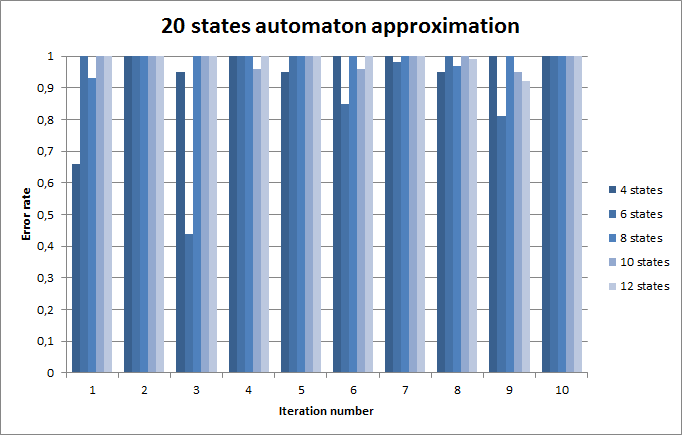
\includegraphics[scale=0.92]{2.png}
\endminipage\hfill
\hspace{2.2cm}
\minipage{0.6\textwidth}
\renewcommand{\arraystretch}{1.3}% Wider
\begin{tabular}{@{}cccccc@{}}
\toprule
        & 4 states & 6 states & 8 states & 10 states & 12 states    \\ \midrule
1       & 0,66     & 1        & 0,93     & 1         & 1 \\
2       & 1        & 1        & 1        & 1         & 1 \\
3       & 0,95     & 0,44     & 1        & 1         & 1 \\
4       & 1        & 1        & 1        & 0,96      & 1   \\
5       & 0,95     & 1        & 1        & 1         & 1   \\
6       & 1        & 0,85     & 1        & 0,96      & 1    \\
7       & 1        & 0,98     & 1        & 1         & 1    \\
8       & 0,95     & 1        & 0,97     & 1         & 0,99     \\
9       & 1        & 0,81     & 1        & 0,95      & 0,92 \\
10      & 1        & 1        & 1        & 1         & 1  \\ \bottomrule
Average & 0,951    & 0,908    & 0,99     & 0,987     & 0,991  \\ \bottomrule
\end{tabular}
\vspace{4mm}
\endminipage\hfill
\caption{Aproksymacja automatu 20-stanowego na zbiorze testowym}
\end{figure}

\begin{figure}[!htb]
\minipage{0.5\textwidth}
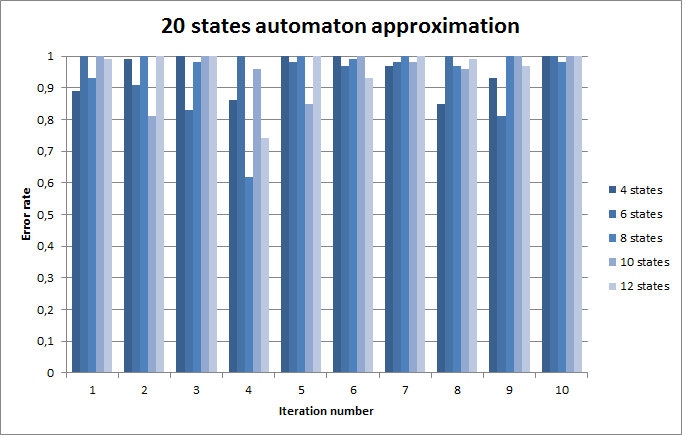
\includegraphics[scale=0.92]{7.png}
\endminipage\hfill
\hspace{2.2cm}
\minipage{0.6\textwidth}
\renewcommand{\arraystretch}{1.3}% Wider
\begin{tabular}{@{}cccccc@{}}
\toprule
        & 4 states & 6 states & 8 states & 10 states & 12 states    \\ \midrule
1       & 0,89     & 1        & 0,93     & 1         & 0,99 \\
2       & 0,99     & 0,91     & 1        & 0,81      & 1 \\
3       & 1        & 0,83     & 0,98     & 1         & 1 \\
4       & 0,86     & 1        & 0,62     & 0,96      & 0,74   \\
5       & 1        & 0,98     & 1        & 0,85      & 1   \\
6       & 1        & 0,97     & 0,99     & 1         & 0,93    \\
7       & 0,97     & 0,98     & 1        & 0,98      & 1    \\
8       & 0,85     & 1        & 0,97     & 0,96      & 0,99     \\
9       & 0,93     & 0,81     & 1        & 1         & 0,97 \\
10      & 1        & 1        & 0,98     & 1         & 1  \\ \bottomrule
Average & 0,949    & 0,948    & 0,947    & 0,956     & 0,962  \\ \bottomrule
\end{tabular}
\vspace{4mm}
\endminipage\hfill
\caption{Aproksymacja automatu 20-stanowego na zbiorze treningowym}
\end{figure}

\FloatBarrier
\subsection{Skuteczność aproksymacji automatu o 30 stanach}

Aproksymacja automatu o 30 stanach automatami o dopowiednio 4, 6, 8, 10 i 12 stanach zakończyła się podobnie do aproksymacji automatu o stanach 20. Warto zauważyć, że analogicznie średni błąd aproksymacji dla zbioru treningowego jest prawie stały na poziomie 0,96. Aproksymacja nieznacznie zwraca większe błędy w porównaniu do automatu o 20 stanach. Poziom błędów można uznać za niesatysfakcjonujący.  \\

\begin{figure}[!htb]
\minipage{0.5\textwidth}
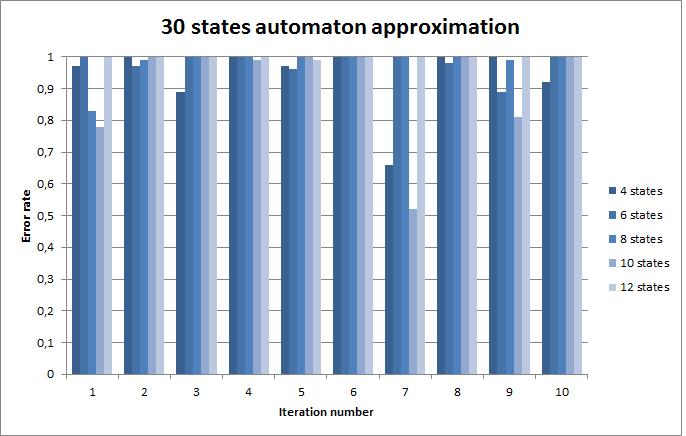
\includegraphics[scale=0.92]{3.png}
\endminipage\hfill
\hspace{2.2cm}
\minipage{0.6\textwidth}
\renewcommand{\arraystretch}{1.3}% Wider
\begin{tabular}{@{}cccccc@{}}
\toprule
        & 4 states & 6 states & 8 states & 10 states & 12 states    \\ \midrule
1       & 0,97     & 1        & 0,83     & 0,78      & 1 \\
2       & 1        & 0,97     & 0,99     & 1         & 1 \\
3       & 0,89     & 1        & 1        & 1         & 1 \\
4       & 1        & 1        & 1        & 0,99      & 1   \\
5       & 0,97     & 0,96     & 1        & 1         & 0,99   \\
6       & 1        & 1        & 1        & 1         & 1    \\
7       & 0,66     & 1        & 1        & 0,52      & 1    \\
8       & 1        & 0,98     & 1        & 1         & 1     \\
9       & 1        & 0,89     & 0,99     & 0,81      & 1 \\
10      & 0,92     & 1        & 1        & 1         & 1  \\ \bottomrule
Average & 0,941    & 0,98     & 0,981    & 0,91      & 0,999  \\ \bottomrule
\end{tabular}
\vspace{4mm}
\endminipage\hfill
\caption{Aproksymacja automatu 30-stanowego na zbiorze testowym}
\end{figure}

\begin{figure}[!htb]
\minipage{0.5\textwidth}
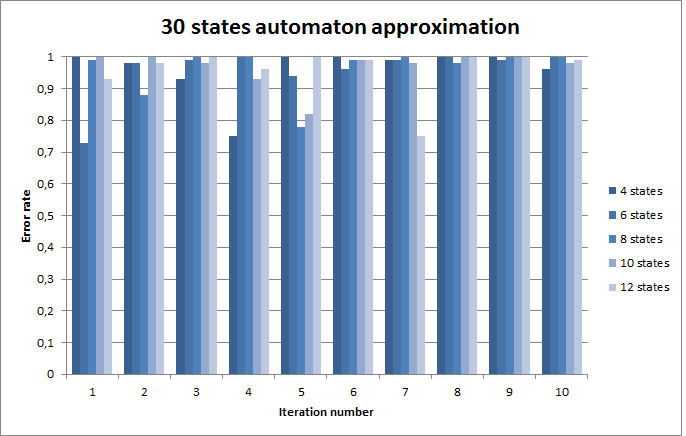
\includegraphics[scale=0.92]{8.png}
\endminipage\hfill
\hspace{2.2cm}
\minipage{0.6\textwidth}
\renewcommand{\arraystretch}{1.3}% Wider
\begin{tabular}{@{}cccccc@{}}
\toprule
        & 4 states & 6 states & 8 states & 10 states & 12 states    \\ \midrule
1       & 1        & 0,73     & 0,99     & 1         & 0,93 \\
2       & 0,98     & 0,98     & 0,88     & 1         & 0,98 \\
3       & 0,93     & 0,99     & 1        & 0,98      & 1 \\
4       & 0,75     & 1        & 1        & 0,93      & 0,96   \\
5       & 1        & 0,94     & 0,78     & 0,82      & 1   \\
6       & 1        & 0,96     & 0,99     & 0,99      & 0,99    \\
7       & 0,99     & 0,99     & 1        & 0,98      & 0,75    \\
8       & 1        & 1        & 0,98     & 1         & 1    \\
9       & 1        & 0,99     & 1        & 1         & 1 \\
10      & 0,96     & 1        & 1        & 0,98      & 0,99  \\ \bottomrule
Average & 0,961    & 0,958    & 0,962    & 0,968     & 0,96  \\ \bottomrule
\end{tabular}
\vspace{4mm}
\endminipage\hfill
\caption{Aproksymacja automatu 30-stanowego na zbiorze treningowym}
\end{figure}

\FloatBarrier
\subsection{Skuteczność aproksymacji automatu o 50 stanach}

Aproksymacja automatu o 50 stanach automatami o dopowiednio 4, 6, 8, 10 i 12 stanach zakończyła się analogicznie dla poprzednich aproksymacji (dla stanów 20 i 30). Warto zauważyć, że analogicznie średni błąd aproksymacji dla zbioru treningowego jest prawie stały na poziomie 0,97. Aproksymacja nieznacznie zwraca większe błędy w porównaniu do automatu o 20 i 30 stanach. Poziom błędów dla zbioru treningowego wynosi prawie 0,98 co powoduje, że wyniki automatu aproksymującego dają złą odpowiedź dla 98 słów ze zbioru 100 słów testowych. Jest to wynik niezadowalający.\\

\begin{figure}[!htb]
\minipage{0.5\textwidth}
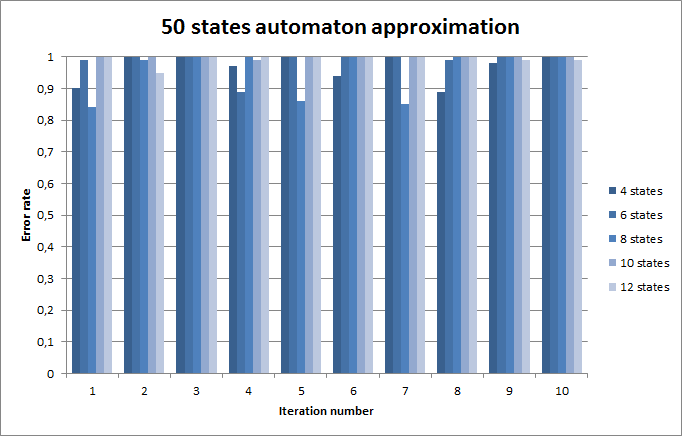
\includegraphics[scale=0.92]{4.png}
\endminipage\hfill
\hspace{2.2cm}
\minipage{0.6\textwidth}
\renewcommand{\arraystretch}{1.3}% Wider
\begin{tabular}{@{}cccccc@{}}
\toprule
        & 4 states & 6 states & 8 states & 10 states & 12 states    \\ \midrule
1       & 0,9      & 0,99     & 0,84     & 1         & 1 \\
2       & 1        & 1        & 0,99     & 1         & 0,95 \\
3       & 1        & 1        & 1        & 1         & 1 \\
4       & 0,97     & 0,89     & 1        & 0,99      & 1   \\
5       & 1        & 1        & 0,86     & 1         & 1   \\
6       & 0,94     & 1        & 1        & 1         & 1    \\
7       & 1        & 1        & 0,85     & 1         & 1    \\
8       & 0,89     & 0,99     & 1        & 1         & 1     \\
9       & 0,98     & 1        & 1        & 1         & 0,99 \\
10      & 1        & 1        & 1        & 1         & 0,99  \\ \bottomrule
Average & 0,968    & 0,987    & 0,954    & 0,999     & 0,993  \\ \bottomrule
\end{tabular}
\vspace{4mm}
\endminipage\hfill
\caption{Aproksymacja automatu 50-stanowego na zbiorze testowym}
\end{figure}

\begin{figure}[!htb]
\minipage{0.5\textwidth}
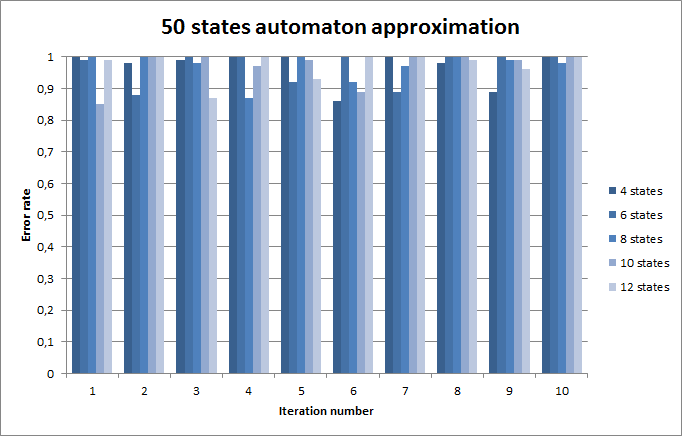
\includegraphics[scale=0.92]{9.png}
\endminipage\hfill
\hspace{2.2cm}
\minipage{0.6\textwidth}
\renewcommand{\arraystretch}{1.3}% Wider
\begin{tabular}{@{}cccccc@{}}
\toprule
        & 4 states & 6 states & 8 states & 10 states & 12 states    \\ \midrule
1       & 1        & 0,99     & 1        & 0,85      & 0,99 \\
2       & 0,98     & 0,88     & 1        & 1         & 1 \\
3       & 0,99     & 1        & 0,98     & 1         & 0,87 \\
4       & 1        & 1        & 0,87     & 0,97      & 1   \\
5       & 1        & 0,92     & 1        & 0,99      & 0,93   \\
6       & 0,86     & 1        & 0,92     & 0,89      & 1    \\
7       & 1        & 0,89     & 0,97     & 1         & 1    \\
8       & 0,98     & 1        & 1        & 1         & 0,99    \\
9       & 0,89     & 1        & 0,99     & 0,99      & 0,96 \\
10      & 1        & 1        & 0,98     & 1         & 1  \\ \bottomrule
Average & 0,97    & 0,968     & 0,971    & 0,969     & 0,974  \\ \bottomrule
\end{tabular}
\vspace{4mm}
\endminipage\hfill
\caption{Aproksymacja automatu 50-stanowego na zbiorze treningowym}
\end{figure}

\FloatBarrier
\subsection{Skuteczność aproksymacji automatu o 80 stanach}

Aproksymacja automatu o 80 stanach podobnie jak dla poprzednich aproksymacji (dla 20, 30 i 50 stanów) zarówno dla zbioru słów treningowych jak i testowych zwraca wyniki niezadowalające. Przy tej aproksymacji można założyć, że współczynnik błędów jest równy 1 dla obu zbiorów. \\

\begin{figure}[!htb]
\minipage{0.5\textwidth}
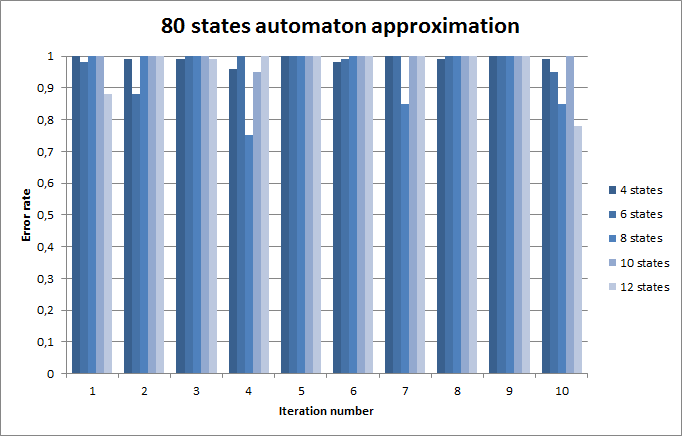
\includegraphics[scale=0.92]{5.png}
\endminipage\hfill
\hspace{2.2cm}
\minipage{0.6\textwidth}
\renewcommand{\arraystretch}{1.3}% Wider
\begin{tabular}{@{}cccccc@{}}
\toprule
        & 4 states & 6 states & 8 states & 10 states & 12 states    \\ \midrule
1       & 1        & 0,98     & 1        & 1         & 0,88 \\
2       & 0,99     & 0,88     & 1        & 1         & 1 \\
3       & 0,99     & 1        & 1        & 1         & 0,99 \\
4       & 0,96     & 1        & 0,75     & 0,95      & 1   \\
5       & 1        & 1        & 1        & 1         & 1   \\
6       & 0,98     & 0,99     & 1        & 1         & 1    \\
7       & 1        & 1        & 0,85     & 1         & 1    \\
8       & 0,99     & 1        & 1        & 1         & 1     \\
9       & 1        & 1        & 1        & 1         & 1 \\
10      & 0,99     & 0,95     & 0,85     & 1         & 0,78  \\ \bottomrule
Average & 0,99     & 0,98     & 0,945    & 0,995     & 0,965  \\ \bottomrule
\end{tabular}
\vspace{4mm}
\endminipage\hfill
\caption{Aproksymacja automatu 80-stanowego na zbiorze testowym}
\end{figure}

\begin{figure}[!htb]
\minipage{0.5\textwidth}
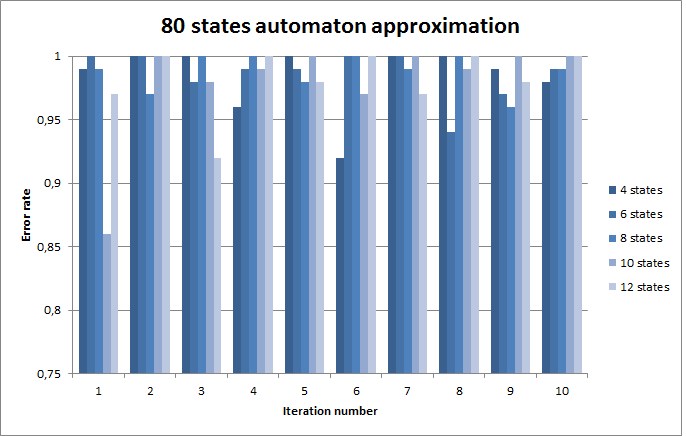
\includegraphics[scale=0.92]{10.png}
\endminipage\hfill
\hspace{2.2cm}
\minipage{0.6\textwidth}
\renewcommand{\arraystretch}{1.3}% Wider
\begin{tabular}{@{}cccccc@{}}
\toprule
        & 4 states & 6 states & 8 states & 10 states & 12 states    \\ \midrule
1       & 0,99     & 1        & 0,99     & 0,86      & 0,97 \\
2       & 1        & 1        & 0,97     & 1         & 1 \\
3       & 1        & 0,98     & 1        & 0,98      & 0,92 \\
4       & 0,96     & 0,99     & 1        & 0,99      & 1   \\
5       & 1        & 0,99     & 0,98     & 1         & 0,98   \\
6       & 0,92     & 1        & 1        & 0,97      & 1    \\
7       & 1        & 1        & 0,99     & 1         & 0,97    \\
8       & 1        & 0,94     & 1        & 0,99      & 1    \\
9       & 0,99     & 0,97     & 0,96     & 1         & 0,98 \\
10      & 0,98     & 0,99     & 0,99     & 1         & 1  \\ \bottomrule
Average & 0,984    & 0,986    & 0,988    & 0,979     & 0,982  \\ \bottomrule
\end{tabular}
\vspace{4mm}
\endminipage\hfill
\caption{Aproksymacja automatu 80-stanowego na zbiorze treningowym}
\end{figure}

\FloatBarrier
\subsection{Podsumowanie i wnioski}

Znalezione automaty przy pomocy algorytmu PSO nie mogą służyć za automaty dobrze aproksymujące automaty wejściowe jeżeli ilość stanów automatu aproksymującego różni się znacznie od ilości stanów automatu aproksymowanego. Wyniki dla automatów o ilości stanów 20, 30, 50 oraz 80 potwierdzają tą tezę. Algorytm sprawdza się dobrze dla małych automatów z podobną ilością stanów co automat wejściowy. Zwiększanie ilości iteracji algorytmu PSO poprawia znacznie współczynnik błędu znalezionego automatu. \\
\end{document}
